\section{Quadratic Discriminant Analysis}
\subsection{Theory}
In some cases, using LDA can be insufficient, since in some cases the data won't be easily deffined as being higher or lower than a linear assumption. In these cases a Quadratic Discriminant Analysis (QDA) can be sufficient. Different from the LDA, the QDA results in a non-linear assumption. The math behind it is given in \ref{fo:quadraticDiscriminantAnalysis1} and \ref{fo:quadraticDiscriminantAnalysis2}.

\begin{align}\label{fo:quadraticDiscriminantAnalysis1}
\delta_k(x) &= - \frac{1}{2} (x - \mu_k)^T \Sigma_{k}^{-1} (x - \mu_k) - \frac{1}{2} \log|\Sigma_{k}| + \log\pi_k\\
			\label{fo:quadraticDiscriminantAnalysis2}
			&= - \frac{1}{2} x^T \Sigma_{k}^{-1} x + x^T \Sigma_{k}^{-1} \mu_k - \frac{1}{2} \mu_k^T \Sigma_{k}^{-1} \mu_k - \frac{1}{2} \log|\Sigma_{k}| + \log\pi_k
\end{align}

Where $\Sigma_{k}$ is a covariance matrix for the \textit{k}th class. Under this assumption, the Bayes classifier assigns an observation $X = x$ to the class for which $\sigma_k$ is largest.

On Figure \ref{fig:linearContraQuadratic} two examples are shown. One using LDA versus QDA on a linear model ($\Sigma_{1} = \Sigma_{2}$), and one using LDA versus QDA on a non-linear model ($\Sigma_{1} \neq \Sigma_{2}$).

\begin{figure}[H]
	\centering
	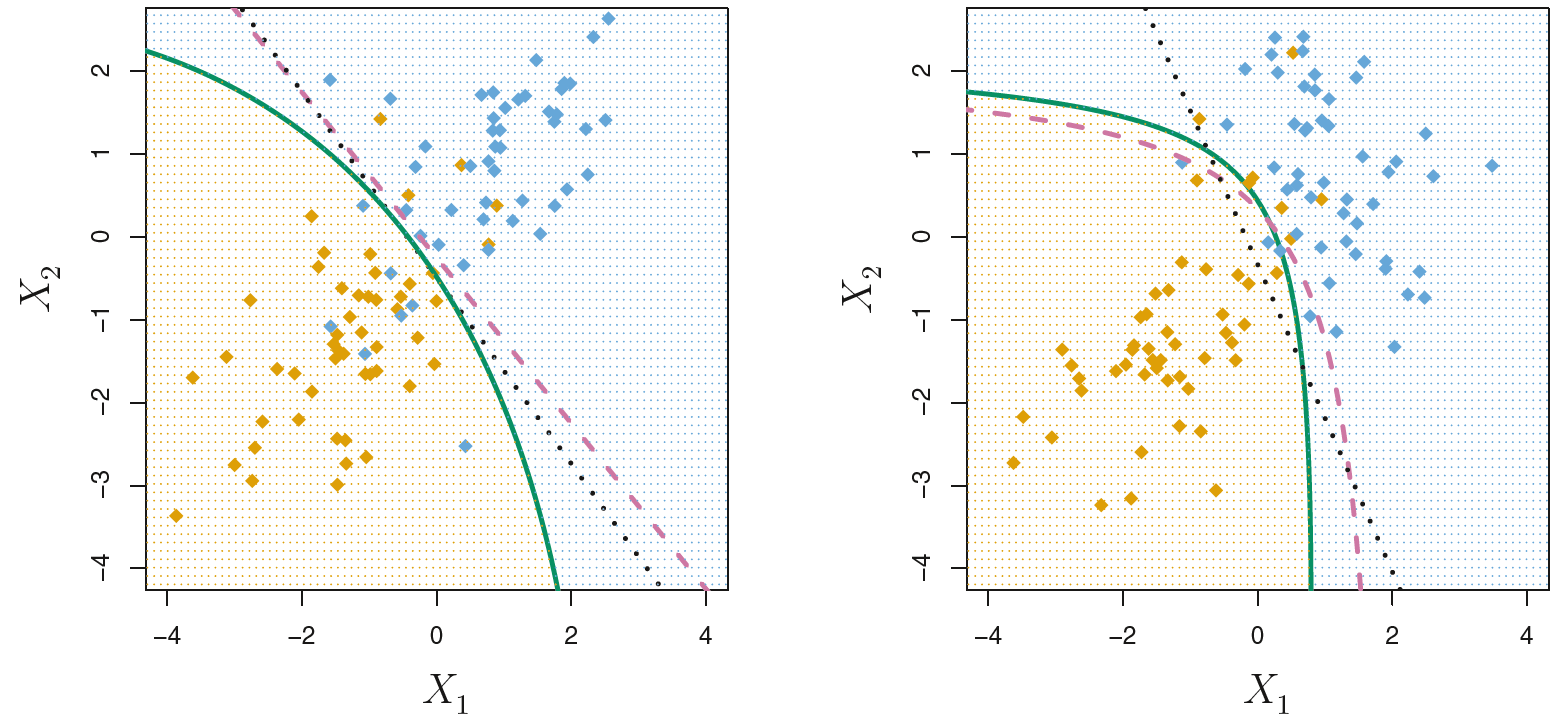
\includegraphics[width=0.7\linewidth]{discriminantAnalysis/quadraticDiscriminantAnalysis/fig/linearContraQuadratic}
	\caption{Purple dash indicate the Bayes, blue dots indicate the LDA, green lines indicate the QDA. On the left the Bayes decision boundary is linear ($\Sigma_{1} = \Sigma_{2}$). On the right the Bayes decision boundary is non-linear ($\Sigma_{1} \neq \Sigma_{2}$)}
	\label{fig:linearContraQuadratic}
\end{figure}

\subsection{Results}
\subsubsection*{LAB 4.6.4}
In lab 4.6.4\footnote{Appendix 6 - 4.6.4 Quadratic Discriminant Analysis} The data is spited as data in lab 4.6.2. The data is split into before and after 2005, a training and testing set.

In the training process only Lag1 and Lag2 is used. Testing the trained model, results in an accuracy of $0.59920634920634919$ approximately $0.60$

The QDA predictions are accurate almost $60\%$ of the time. This shows that the Quadratic Discriminant Analysis seem to capture the relationship more accurately than the Linear Discriminant Analysis. The output contains the group means. But it does not contain the coefficients of the linear discriminants, because the QDA classifier involves a quadratic, rather than a linear, function of the predictors.

The results are seen in the table below.

\begin{longtable}[]{@{}lll@{}}
	\toprule
	& Lag1 & Lag2\tabularnewline
	\midrule
	\endhead
	Down & 0.04279022 & 0.03389409\tabularnewline
	Up & -0.03954635 & -0.03132544\tabularnewline
	\bottomrule
\end{longtable}